\section{目的與講義對照}

依講義 PDF 第 62--64 頁完成步驟 1 的 FF／TT／SS 延遲與功率比較，問題 1 的混合角落 ratioed logic 比較，以及問題 2 的反偏接面漏電比較。共 8 份網表、17 個實際分析。

本實驗依使用者選定的 CIC 0.18 µm、1.8 V 元件進行；講義原範例是 0.25 µm、2.5 V，因此結果不是原表格的數值重現。保留講義反相器尺寸 Wn/Wp/L = 0.6/1.8/0.25 µm，名義供應改為 1.8 V。1.98 V 與 1.62 V 為明列的正負 10\% 教學角落條件；這不等同電壓可靠度認證。

\section{方法與可重現資料}

使用 HSPICE S-2021.09，所有分析完成且未回報 warning、error 或 failed measurement。輸入週期 4 ns、rise/fall 0.2 ns，輸出負載 10 fF；延遲使用第二次邊緣的半供應電壓交越，$t_p=(t_{pHL}+t_{pLH})/2$。功率為 4--12 ns 的平均電源輸入功率。FF、SS 各增加 1.8 V、25°C 的分析以分離製程變化。

網表 01--03 為 transient，04--08 為 DC。公開網表僅保留 \texttt{MODEL\_SETUP\_REQUIRED} 與角落名稱註解；模型內容及載入路徑不隨檔案發布，執行前須補入本機設定。所有圖由實際模擬資料繪製；\texttt{results/} 附逐案例 CSV、量測 JSON 與比較 CSV。

\section{製程、電壓與溫度結果}

\begin{center}\small
\begin{tabular}{lrrrr}
\toprule
Corner & V (V) & T (°C) & $t_p$ (ps) & $P$ (µW) \\
\midrule
TT & 1.8 & 25 & 87.110 & 11.946 \\
FF & 1.98 & 0 & 69.853 & 15.239 \\
SS & 1.62 & 115 & 159.081 & 10.150 \\
FF & 1.8 & 25 & 77.092 & 12.240 \\
SS & 1.8 & 25 & 129.262 & 12.232 \\
\bottomrule
\end{tabular}
\end{center}

\begin{figure}[htbp]\centering
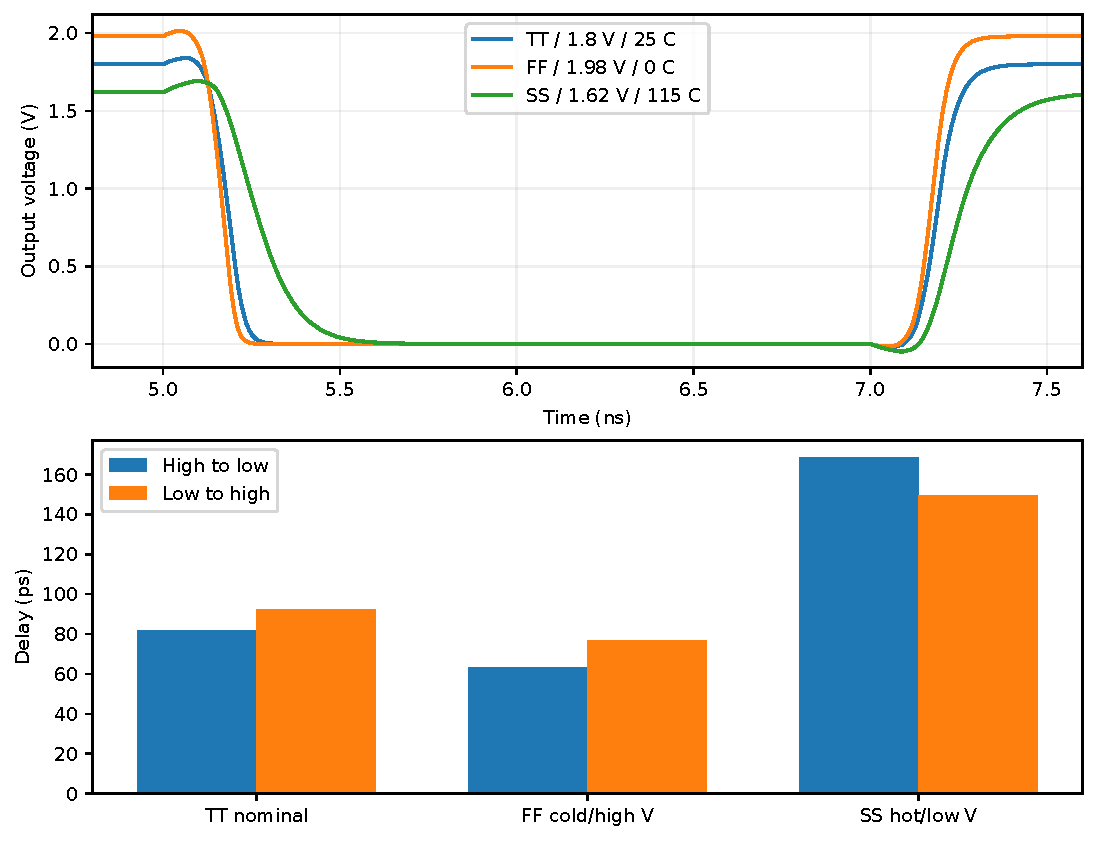
\includegraphics[width=.93\linewidth]{figures/pvt.pdf}
\caption{前三個合併 PVT 案例的輸出與兩種傳播延遲。}
\end{figure}

合併角落的平均延遲依 FF、TT、SS 為 69.853、87.110、159.081 ps；功率為 15.239、11.946、10.150 µW，符合此組條件下快角落較快且較耗電的趨勢。但固定電壓與溫度時，SS 功率 12.232 µW 略高於 TT，顯示功率不能只按 fast/slow 標籤單調排序。輸入頻率、負載充放電與短路電流都會影響結果。

\section{問題 1：ratioed logic 的混合角落}

Pseudo-NMOS 的 PMOS 永遠導通，尺寸 0.6/0.5 µm；NMOS 為 0.6/0.25 µm。低電位由上拉與下拉電流平衡決定，故需要檢查 SF、FS。下表為 1.8 V、25°C、輸入 1.8 V；靜態 CMOS 的低電位均接近 0，pseudo-NMOS 則保留可見的直流壓降及功耗。

\begin{center}\small
\begin{tabular}{lrr}
\toprule
Corner & $V_{OL}$ (V) & $P_{static}$ (µW) \\
\midrule
TT & 0.063495 & 87.209 \\
FF & 0.061252 & 102.027 \\
SS & 0.100317 & 62.364 \\
SF & 0.172730 & 101.363 \\
FS & 0.077670 & 93.937 \\
\bottomrule
\end{tabular}
\end{center}

\begin{figure}[htbp]\centering
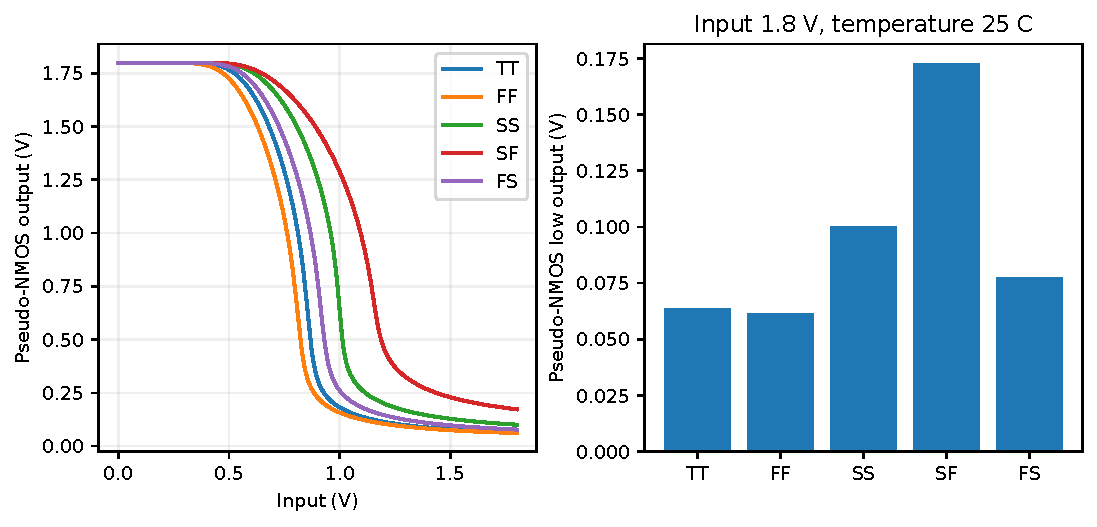
\includegraphics[width=.93\linewidth]{figures/ratioed.pdf}
\caption{混合角落造成 ratioed 電路低電位最差點改變。}
\end{figure}

本次 SF 的 VOL = 0.172730 V，高於 FF、TT、SS，因此僅檢查三個同向角落會漏掉此項最差結果。對靜態 CMOS 而言，ratio-less 並不代表 SF/FS 永遠不必驗證；切換點、占空比、雜訊容限或其他不對稱規格仍可能受混合角落限制。

\section{問題 2：反偏接面漏電}

另建 NMOS 與 PMOS，D、S、G 短接，使 $V_{DS}=V_{GS}=0$，只反偏兩個 D/B、S/B 接面。每個接面面積 0.15 µm$^2$、周長 1.7 µm，反偏 1.8 V。量測 body 電流，分開列出兩接面總和；沒有把整個反相器的 off-state 電流誤稱為單一接面漏電。

採用 GMIN = GMINDC = $10^{-18}$ S，兩接面的數值導通貢獻為 $2(1.8)(10^{-18})=3.6\times10^{-18}$ A，從 raw 值明確扣除。另以 $10^{-15}$ S 重跑 TT、25°C，扣除後 NMOS 與 PMOS 均回到相同數值；保留 raw 與校正值於 CSV。0°C 的 raw 值很小，數值導通占比不可忽略。

\begin{center}\small
\begin{tabular}{lrr}
\toprule
T (°C) & N (A) & P (A) \\
\midrule
0 & 4.7115e-18 & 2.8546e-18 \\
25 & 4.2894e-16 & 2.5988e-16 \\
115 & 4.9026e-11 & 2.9704e-11 \\
\bottomrule
\end{tabular}
\end{center}

\begin{figure}[htbp]\centering
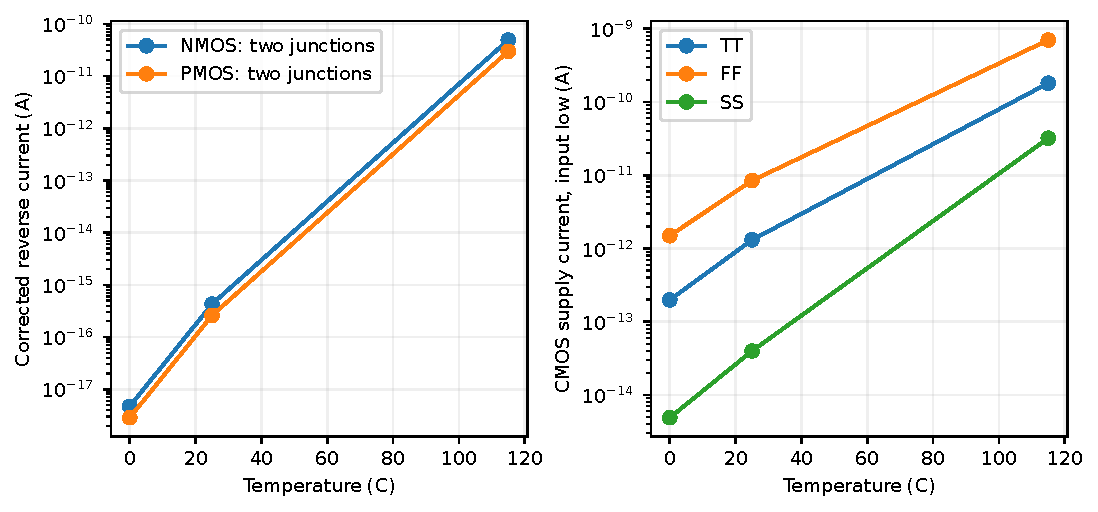
\includegraphics[width=.93\linewidth]{figures/leakage.pdf}
\caption{左：校正接面漏電；右：反相器供應漏電，兩者不是相同量。}
\end{figure}

此模型在相同溫度及接面幾何下，TT／FF／SS 的隔離接面電流相同；溫度造成極大的變化。另一方面，反相器供應漏電會隨角落改變，例如 25°C、輸入低時 FF/TT/SS 分別為 8.429/1.308/0.03975 pA。故不能假設所有漏電機制都具有 FF > TT > SS 的相同排序。

\section{結論與限制}

已完成講義的角落延遲、功耗及兩個問題。結果僅對此模型、尺寸、負載與明列刺激成立；未宣稱原 0.25 µm 數值重現、完整 PVT 簽核、統計良率或版圖後模擬。沒有在本實驗改動其他 lab 的模型。
